

\section{Dataset and Study Area}

A pair of co-registered L-band ($\lambda = 0.23m$) UAVSAR images acquired over Los Angeles, California in 23-04-2009 and 11-05-2015 respectively  with a resolution of $0.4m$ in azimuth and $1.66m$ in range are used in this study. The dataset is multi-looked $2\times8$ times to form an effective pixel-size of $3.2m$.  The study-area is a dense urban area with changes occurring primarily due to the effects of urbanization. 

The objective of the proposed methodology is to  characterize the construction and destruction of urban areas, while simultaneously classifying unchanged urban and natural areas in the rest of the scene.
The major changes, i.e. `Changed Urban' class observed include the construction of suburban neighborhoods, industrial structures and public infrastructure like rail-yards and airports.  Natural areas of vegetation  comprise of the `Natural Unchanged' class. The urban infrastructure like houses, buildings, roads etc. that did not change is the 'Urban Unchanged' class.
%Thus the classes "Changed Urban" This represents both the changed urban areas and a land-cover classification of the unchanged areas: simultaneously generating an urban change and extent map.

%\section{Experimental Results and Discussion}
\section{Experimental Set-Up}
\label{sec:exp}
The images are pre-processed and stacked to form the 20 dimensional input vector $x$.  The AE is a sparse 7-layer network comprised of 512, 256, 128 nodes in the encoder, 8 in the representational layer and 128, 256, 512 in the decoder with ReLU nodes. The auto-encoder is trained in an unsupervised manner with learning rate $\alpha=1e-5$ at initialization and is dropped by a step factor of $\Gamma=0.1$ every $100,000$ iterations.  After training,  $z$ is extracted from the representational layer and a PCA is applied pixel wise. It is seen that $k=3$ principal components contain most of the useful information.
% activation function used is ReLU. The learning rate $\alpha=1e-5$ at initialization and is dropped by a step factor of $\Gamma=0.1$ every $100,000$ iterations.

\begin{figure}
\centering
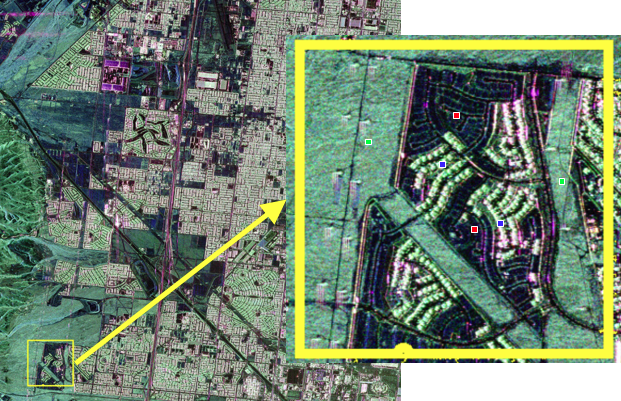
\includegraphics[width = 0.7\textwidth]{Figures/CD/ADD/plot}
\caption{Map of all the ground reference information used for CD. As can be seen, the reference information is minimal, and constrained to a small spatial area of the scene.}
\label{fig:const}
\end{figure}

In a realistic scenario, reference information about the scene would only be available in a small portion of the area. Hence training samples are drawn from the part of the scene bounded by the yellow square in Figure~\ref{fig:2_a}. For each class $20$ pixels are labeled based on prior knowledge of the region and optical imagery as shown in Figure~\ref{fig:const}. A total of $l=60$ training samples are  used, and $l<<N=9e6$ making the problem weakly supervised. A label aggregation step is performed by the ellipsoidal fitting technique described above. Reservoir sampling is performed to select $L=300$ labeled pixels per class from the points bounded by each ellipsoid. These aggregated labels are used to train a 3-layer MLP network with sigmoid activation function in a supervised manner. The final classification output   is shown in Figure~\ref{fig:2} along with the Pauli composition of the image pair. The output simultaneously maps areas of changed urban ares, unchanged built-up and  natural land-cover. This is an improvement over outputs from  traditional ratio based methods that are unable to leverage the polarimetric information. 

\section{Results and Discussion}
\label{sec:resultsA1}

\begin{figure}[tbp]
\centering
\begin{subfigure}[b]{0.32\textwidth}
		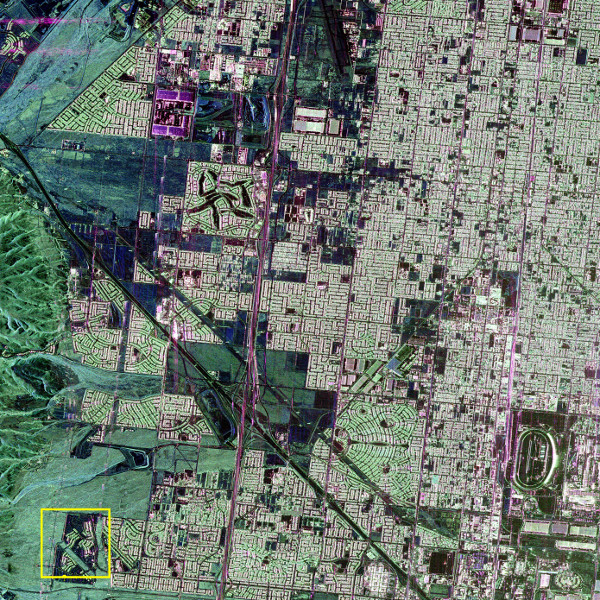
\includegraphics[width=\textwidth]{Figures/CD/2009}
		\caption{}
		\label{fig:2_a}
\end{subfigure}
\hspace{0.05pt}
\begin{subfigure}[b]{0.32\textwidth}
		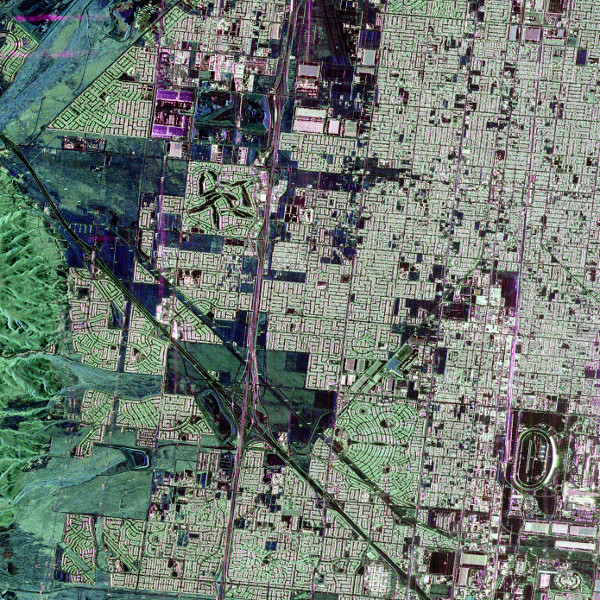
\includegraphics[width=\textwidth]{Figures/CD/2015.jpg}
		\caption{}
		\label{fig:2_b}
\end{subfigure}
\hspace{0.05pt}
\begin{subfigure}[b]{0.32\textwidth}
		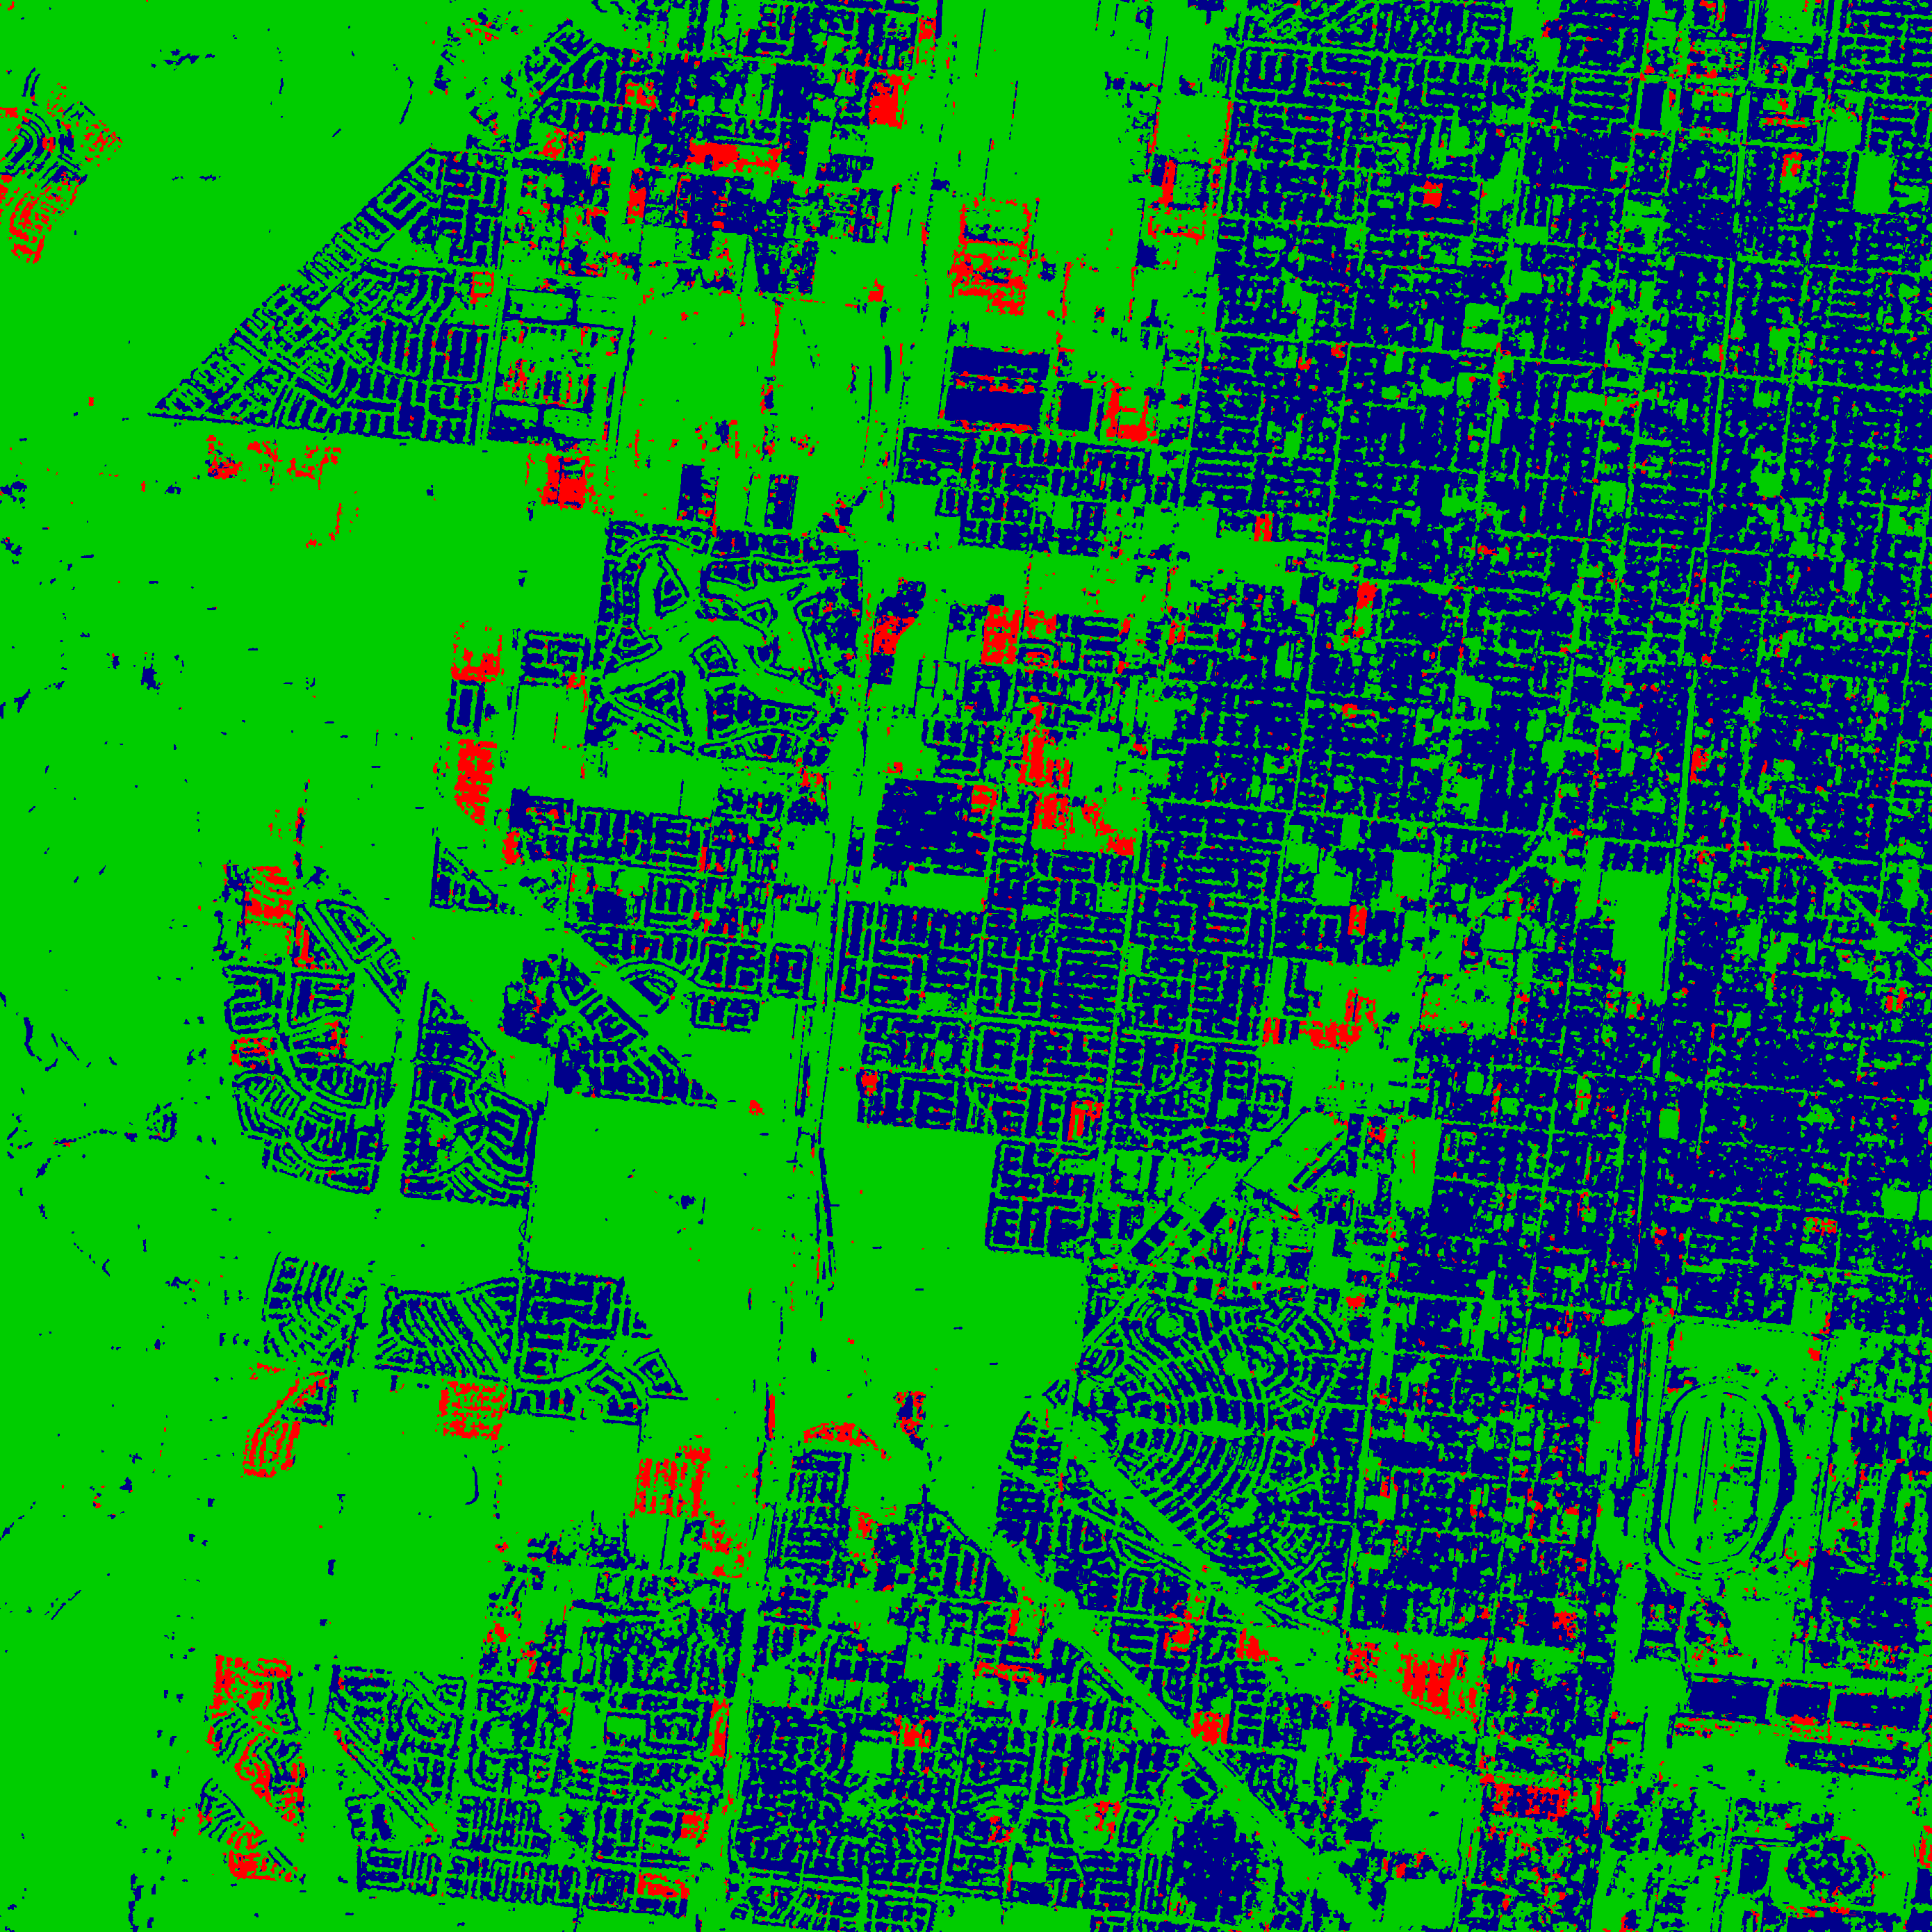
\includegraphics[width=\textwidth]{Figures/CD/result}
		\caption{}
		\label{fig:2_c}
\end{subfigure}

%\hspace{0.05pt}
\begin{subfigure}[b]{\textwidth}
\centering
		\vspace{0.2em}
		\begin{tabular}{ c l  c l  c l  }
	%	\hline
		 
\includegraphics[width=0.01\columnwidth]{Figures/CD/RED} & Urban Change (UC)  \hspace{1mm} &
		 
\includegraphics[width=0.01\columnwidth]{Figures/CD/GREEN} & Natural Unchanged (NU) \hspace{1mm} &
		 
\includegraphics[width=0.01\columnwidth]{Figures/CD/BLUE} & Urban Unchanged (UU) \hspace{1mm} \\
	%	\hline
		\end{tabular}
		%\vspace{20mm}
		%\caption{}
\end{subfigure}
\caption{The Pauli composite of (a) 2009, (b) 2015 image, and (c) the result of the classification. }
\label{fig:2}
\end{figure}



\begin{figure}[tbp]
\centering
\begin{subfigure}[b]{0.7\textwidth}
		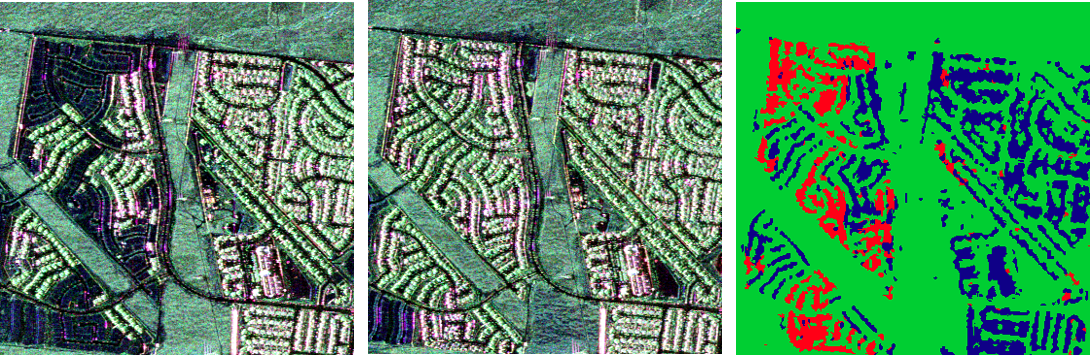
\includegraphics[width=\textwidth]{Figures/CD/ADD/1}
		\caption{}
\end{subfigure}

\begin{subfigure}[b]{0.7\textwidth}
		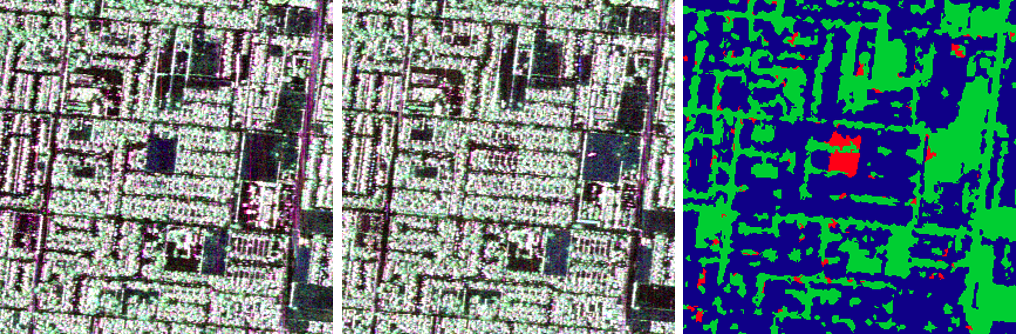
\includegraphics[width=\textwidth]{Figures/CD/ADD/2}
		\caption{}
\end{subfigure}

\begin{subfigure}[b]{0.7\textwidth}
		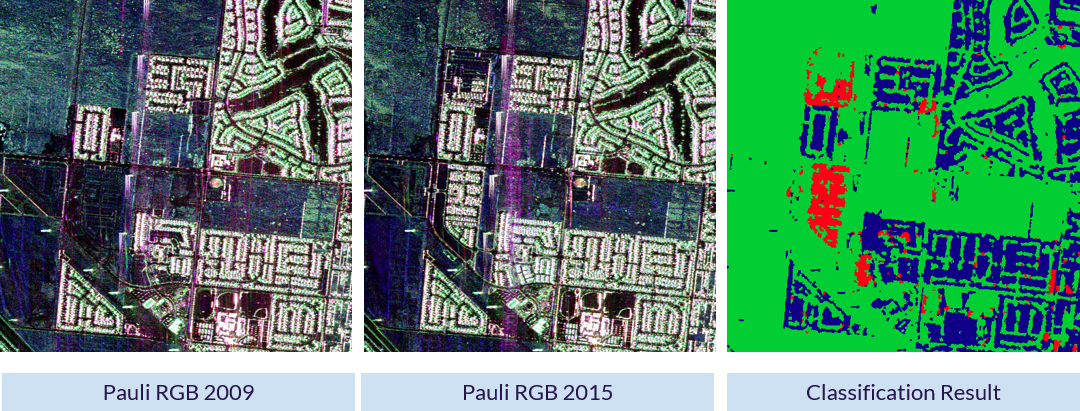
\includegraphics[width=\textwidth]{Figures/CD/ADD/3}
		\caption{}
\end{subfigure}

%\hspace{0.05pt}
\begin{subfigure}[b]{\textwidth}
\centering
		\vspace{0.2em}
		\begin{tabular}{ c l  c l  c l  }
	%	\hline
		 
\includegraphics[width=0.01\columnwidth]{Figures/CD/RED} & Urban Change (UC)  \hspace{1mm} &
		 
\includegraphics[width=0.01\columnwidth]{Figures/CD/GREEN} & Natural Unchanged (NU) \hspace{1mm} &
		 
\includegraphics[width=0.01\columnwidth]{Figures/CD/BLUE} & Urban Unchanged (UU) \hspace{1mm} \\
	%	\hline
		\end{tabular}
		%\vspace{20mm}
		%\caption{}
\end{subfigure}

\caption{From left to right, the Pauli composite of the 2009 and 2015 images, along with the result of the classification is presented for areas (a) A, (b) B and (c) C. }
\label{fig:detail}
\end{figure}


\begin{figure}[t]
\centering
\begin{subfigure}[b]{0.23\columnwidth}
		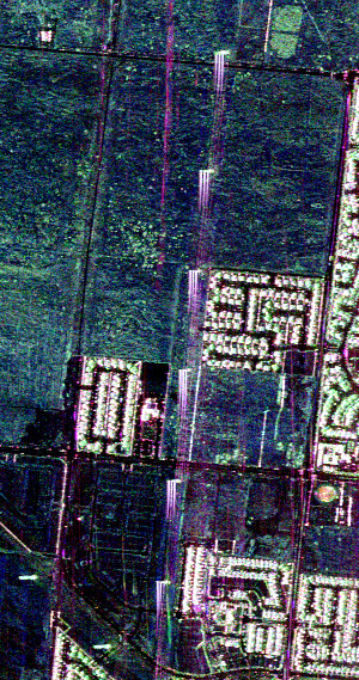
\includegraphics[width=\textwidth]{Figures/CD/A2_2009}
		\caption{}
		\label{fig:3_a}
\end{subfigure}
\hspace{0.01pt}
\begin{subfigure}[b]{0.23\columnwidth}
		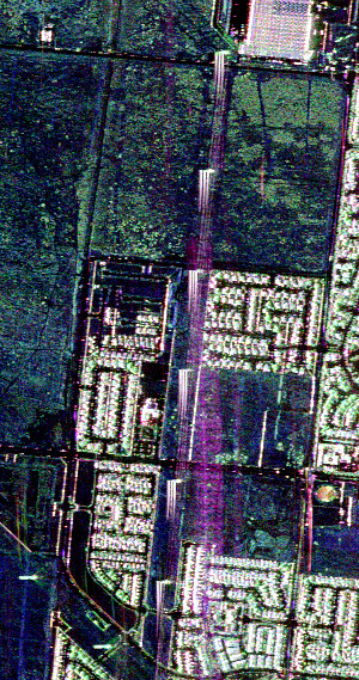
\includegraphics[width=\textwidth]{Figures/CD/A2_2015}
		\caption{}
		\label{fig:3_b}
\end{subfigure}
\hspace{0.01pt}
\begin{subfigure}[b]{0.23\columnwidth}
		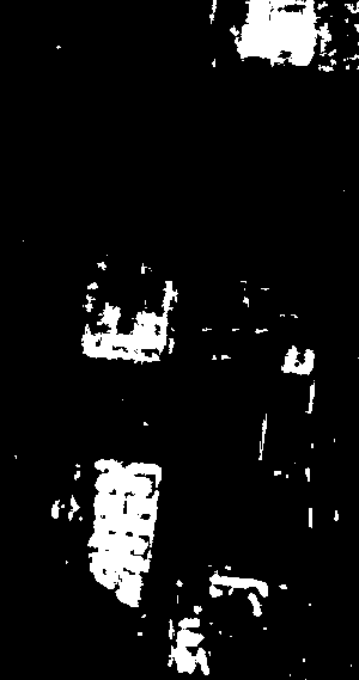
\includegraphics[width=\textwidth]{Figures/CD/REF_A2}
		\caption{}
		\label{fig:3_c}
\end{subfigure}
\hspace{0.01pt}
\begin{subfigure}[b]{0.23\columnwidth}
		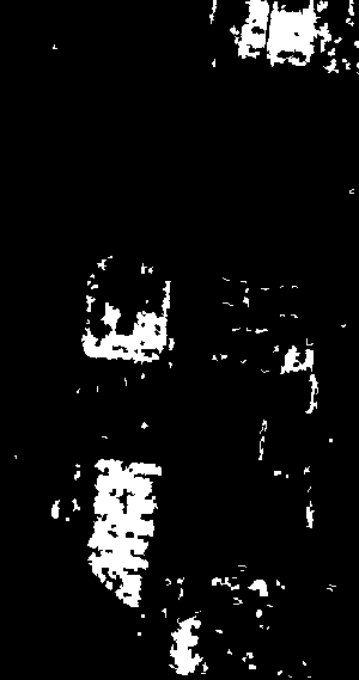
\includegraphics[width=\textwidth]{Figures/CD/OP_1_A2}
		\caption{}
		\label{fig:3_c}
\end{subfigure}

\begin{subfigure}[b]{\columnwidth}
\centering
		\vspace{0.2em}
		\begin{tabular}{c l  c l  }
		 
\includegraphics[width=0.02\columnwidth]{Figures/CD/BLK} & No Change   &
		 
\includegraphics[width=0.02\columnwidth]{Figures/CD/WHT} & Change
		\end{tabular}
\end{subfigure}
\caption{The Pauli composite of detail (a) 2009, (b) 2015 image, and the (c) reference change map, and (d) output change map.}
\label{fig:3}
\end{figure}



Qualitatively, the  output corresponds well with the changed areas observed in the Pauli composition image pair and has low misclassification as shown in Figure~\ref{fig:2}. Comparative crops are shown in Figure~\ref{fig:detail} for three areas of the image. Area 'A' is located close the near range of the radar, and hence is subject to radiometric anomalies due to the steep look angle of the radar, as common with airborne sensors. Despite this, the proposed method performs reasonably well and resilient to the amplitude gradient of the backscatter. The changes in area 'B' are very minor compared to the rest of the area. There is a construction of new housing that has occurred in the vacant lot amidst other built-up areas. The challenge in this crop is that it is close to a train station (right edge), and due to the movement of infrastructure there is inconsistent radar backscatter between the two images. The proposed method is able to capture the change perfectly, ignoring the interference from the railway station. Area 'C' radar artifacts due to return from power-lines can be observed in the two images. Also, the natural areas surrounding the urban structures are significantly changed. The parcel based approach employed in the proposed methodology is able to counter the effects of the artifacts. The method is also able to segregate urban changes from natural ones, something that would not be possible with a traditional change index methodology.     

Quantitatively, 
the confusion matrix is computed and presented in Table~\ref{tab:conf}.  The overall accuracy $OA = 92.34\%$ with $\kappa = 0.88$. The urban change (UC) areas are most commonly confused with the urban unchanged (UU) ones. This corresponds to areas where the learned representation was not sufficient to discriminate the two.
Another source of confusion is between natural unchanged (NU) and UU classes. The presence of vegetation intermixed with buildings in the UU areas makes it more difficult to discern it from the NU class leading to misclassification.
%The Pauli composition of the two images are shown in Figure~\ref{fig:3} with the 






To evaluate the CD capabilities the two unchanged classes, i.e. UU and NU are grouped together as a single unchanged class, with the UC representing the change as shown in Figure~\ref{fig:3}. Performance is evaluated in terms of false positive rate (PFP), false negative rate (PFN), false alarm rate (FA(\%)), detection rate (DR(\%)) and kappa (Table~\ref{tab:cd}). The method has a low FA rate of $FA=2.64\%$. This is due to design of the AE loss function and the radial thinning performed in the label aggregation step. The $DR=82.3\%$ can be improved at the cost of a higher $FA$, by eliminating the radial thinning step during label aggregation. The $\kappa=0.83$ indicates that there is very good agreement between the reference and output maps. This is confirmed qualitatively by visual inspection of the output image. 


\begin{figure}[t]
\centering
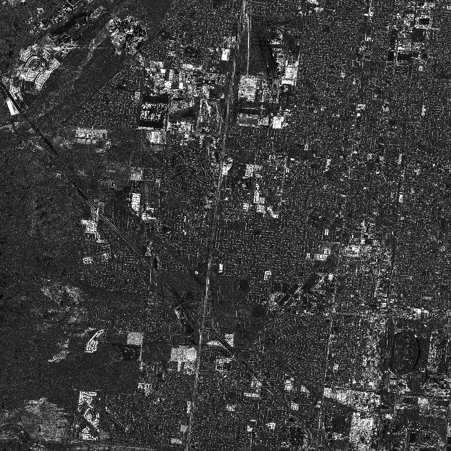
\includegraphics[width = 0.6\textwidth]{Figures/CD/ADD/Diff}
\caption{A traditional log-ratio change index generated for the dataset.}
\label{fig:difflr}
\end{figure}


Figure~\ref{fig:difflr} depicts a traditional log-ratio change index computed on the dataset. The index can reasonably capture the change in the scene, but the original scattering mechanism information is discarded. This prevents simultaneous land-cover classification from being performed. To obtain both the change and land-cover map, two separate processes must be run on the dataset consuming time and computing resources. In contrast, the proposed method is able to efficiently compute both the maps in one go. 

Further, the change index is unable to differentiate between natural and urban changes and only captures the magnitude of the change, disregarding scattering information. Thus, it identifies both the natural and urban changes in the scene as a change, and further analysis is needed to be able to identify the change. In the proposed method, the changes are encoded in the representational layers of the AE, which is then projected in a manifold. Because the scattering information is encoded inherently in this representation, each region of the space corresponds to a particular transition of scattering mechanism between the two images. Due to this it is possible to not only identify the original land cover classes, but also the change information in one step. In a work-flow where a large number of scenes must be automatically processed, this computational advantage can translate to time and resource savings.

\begin{table}
	\centering
	\caption{Confusion Matrix}
	\label{tab:conf}
	\begin{tabular}{cccc|c}
		&  UC (\%)  & NU (\%) & UU (\%) & Total \\ \hline
		UC (\%) & 90.28 & 0.34 &  0.00 & 26.11 \\
		NU (\%) & 2.24 & 88.54 & 1.10  & 35.91\\
		UU (\%) & 7.47 & 11.12 & 98.90 & 37.97\\ \hline
		OA   & 92.34\% &  $\kappa$   & 0.88 & \\ 
	\end{tabular}
	
\end{table}
\begin{table}
	\centering
	\caption{Change Detection Metrics}
	\label{tab:cd}
	\begin{tabular}{c c c c c c}
		PFP(\%)  & PFN(\%) & FA(\%) & DR(\%) & $\kappa$ \\ \hline
		0.89 & 1.75 & 2.64 & 82.3 & 0.83 \\
	\end{tabular}
\end{table}



\subsubsection{Comparative Analysis}

\begin{figure}[t]
\centering
\begin{subfigure}[b]{0.18\columnwidth}
		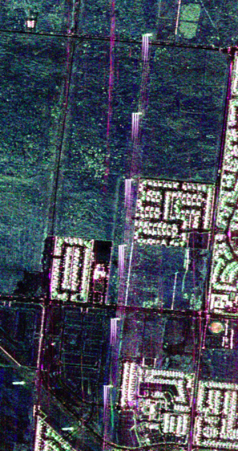
\includegraphics[width=\textwidth]{Figures/CD/ADD/a}
		\caption{}
\end{subfigure}
\hspace{0.01pt}
\begin{subfigure}[b]{0.18\columnwidth}
		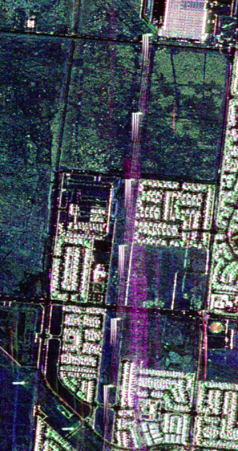
\includegraphics[width=\textwidth]{Figures/CD/ADD/b}
		\caption{}
\end{subfigure}
\hspace{0.01pt}
\begin{subfigure}[b]{0.18\columnwidth}
		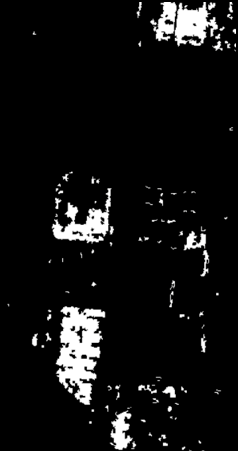
\includegraphics[width=\textwidth]{Figures/CD/ADD/c}
		\caption{}
\end{subfigure}
\hspace{0.01pt}
\begin{subfigure}[b]{0.18\columnwidth}
		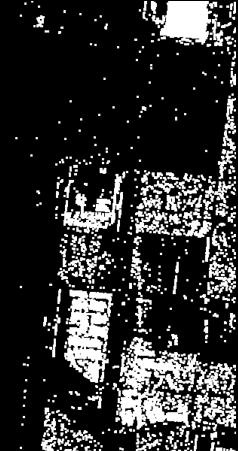
\includegraphics[width=\textwidth]{Figures/CD/ADD/d}
		\caption{}
\end{subfigure}
\hspace{0.01pt}
\begin{subfigure}[b]{0.18\columnwidth}
		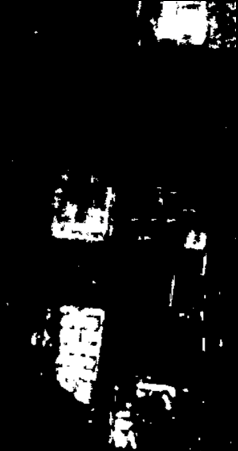
\includegraphics[width=\textwidth]{Figures/CD/ADD/e}
		\caption{}
\end{subfigure}

\begin{subfigure}[b]{\columnwidth}
\centering
		\vspace{0.2em}
		\begin{tabular}{c l  c l  }
		 
\includegraphics[width=0.02\columnwidth]{Figures/CD/BLK} & No Change   &
		 
\includegraphics[width=0.02\columnwidth]{Figures/CD/WHT} & Change
		\end{tabular}
\end{subfigure}
\caption{The Pauli composite of detail (a) 2009, (b) 2015 image, and the result of change detection by (c) proposed and (d) geodesic distance methods, shown along with the (e) reference map.}
\label{fig:comparedeb}
\end{figure}

\begin{table}[]
\centering
\caption{Comparison with other methods}
\label{tab:comparedebanshu}
\begin{tabular}{l|llll}
Approach             & Overall Accuracy & Kappa &  &  \\ \hline
Geodesic Distance (GD)~\cite{ratha2017change}    & 89.20            & 0.78  &  &  \\
Proposed             & 92.34            & 0.88  &  & 
\end{tabular}
\end{table}

The proposed methodology is compared with another recent PolSAR change detection technique~\cite{ratha2017change}. The results are tabulated in Table~\ref{tab:comparedebanshu} and shown in Figure~\ref{fig:comparedeb}. The proposed method is able to outperform the contemporary technique, with an overall accuracy of $92.34\%$ and $\kappa=0.88$. The section of image used in the comparison is fairly challenging for a change detection algorithm due to the presence of power-lines in the scene. These have a very strong radar return, saturating the receiver and leading the artifacts in the image, as seen. Since both the algorithms use variation in the scattering mechanism to identify changes, they are able to successfully avoid the interference of these power-lines. In contrast, change index and amplitude difference based techniques would be susceptible to this nature of interference. 

However, the geodesic distance (GD) measure is still sensitive to changes in natural areas. Over time, vegetation will grow and change, leading to a variation in the observed scattering mechanism. Since the final output is obtained by applying a single threshold to the GD value, it is not possible to fully separate the natural changes from urban ones. In contrast, the proposed method uses ellipsoid fitting to improve the separation of urban changes in the feature space itself. This is followed by a MLP layer, which is further able to flexibly threshold the images to reduce the effect of natural changes. 
%
The region growing in the feature space and parcel based approach at input, combined lead to a very low false alarm rate of $2.64\%$ in the proposed technique, and often in practical application of change detection, a lower false alarm rate is more critical than a high accuracy. 

It must be noted that although the proposed technique outperforms the GD method, it is much more computationally complex. The training phase of the AE is also time consumptive, however, once trained, the final classification can be performed fast. In contrast, the GD method is computationally simple, and can be computed much quicker, at the cost of a slightly lower accuracy and higher false alarm rate. 

%[[156301   1001]
% [  2844  10854]]
%[[ 0.99363644  0.00636356]
% [ 0.20762155  0.79237845]]
%Overall accuracy:
%97.7514619883
%Kappa:
%0.83744617901